\documentclass[12pt, a4paper]{article}
\usepackage{fullpage}
\usepackage{graphicx}
\usepackage{amsmath, amssymb, amsthm, amsfonts}
\usepackage{hyperref}
\usepackage{verbatim}

\usepackage{tikz}
\usetikzlibrary{shapes,arrows,positioning,decorations,decorations.markings}

\newcommand{\tr}{\text{trace}}
\newcommand{\p}{\partial}
\newcommand{\pp}[2]{{\partial #1 \over \partial #2}}
\newcommand{\ppn}[3]{{\partial^{#1} #2 \over \partial #3^{#1}}}
\newcommand{\CC}{\mathbb{C}}
\newcommand{\NN}{\mathbb{N}}
\newcommand{\QQ}{\mathbb{Q}}
\newcommand{\RR}{\mathbb{R}}
\newcommand{\ZZ}{\mathbb{Z}}
\newcommand{\ud}{\,\mathrm{d}}

\newtheorem{theorem}{Theorem}
\newtheorem{definition}{Definition}

\title{
  Stationary Solutions to KdV \\
  {\textsc Reading Group 2010--2011}}
\author{
  Ben Lansdell \\
  Natalie Sheils \\
  Chris Swierczewski}



%%%%%%%%%%%%%%%%%%%%%%%%%%%%%%%%%%%%%%%%%%%%%%%%%%%%%%%%%%%%%%%%%%%%%%%%%%%%%%%
\begin{document}
%%%%%%%%%%%%%%%%%%%%%%%%%%%%%%%%%%%%%%%%%%%%%%%%%%%%%%%%%%%%%%%%%%%%%%%%%%%%%%%

\maketitle

\tableofcontents

\newpage

%==============================================================================
\section{The KdV hierarchy}
%==============================================================================



We first construct the KdV heirarchy by considering the compatibility
condition of two linear evolution systems. We will consider KdV given
by
\[
  4u_t = 6uu_x + u_{xxx},
\]
(subscripts denote partial derivatives) with the associated Lax Pair:

\begin{equation}\label{lax}
  \begin{split}
    \psi_x &= X \psi = \left(
      \begin{array}{cc}
        0 & 1 \\ \lambda-u & 0
      \end{array}
      \right) \psi \\
    \psi_{t_n} &= T_n\psi = \left(
    \begin{array}{cc}
      a_n & b_n \\ c_n & d_n
    \end{array}
    \right)\psi.
  \end{split}
\end{equation}
Note that if $\psi = \left( \begin{smallmatrix}{c} \psi
  \\ \psi_x \end{smallmatrix} \right)$ then $X$ is the Schr\"odinger
operator with potential function $u(x)$ and energy $\lambda$.

We impose a compatibility condition $\psi_{x t_n}=\psi_{t_n x}$ or
\begin{equation*}
  X_{t_n} + X T_n = T_{nx} + T_n X,
\end{equation*}
or
\begin{equation*}
  \left(
  \begin{array}{cc}
    c - a_x - (\lambda - u) b & d - b_x - a \\
    (\lambda - u)(a - d) - u_{t_n} - c_x & (\lambda - u) b - d_x - c
  \end{array}
  \right) = 0,
\end{equation*}
where we have dropped the subscript $n$ on $a,b,c,d$ for convenience.

Componentwise this gives us,
\begin{align*}
  a_x &= c - (\lambda - u) b \\
  b_x &= d - a \\
  c_x &= (\lambda - u)(a - d) - u_{t_n} \\
  d_x &= -c + (\lambda - u) b.
\end{align*}

Note that $a_x = -d_x$.  We pick $d = -a$.  Integrating the equations
above we have, in terms of $b$ and its derivatives,
\begin{align}
  a &= -\frac{1}{2} b_x \notag \\
  c &= (\lambda - u) b - \frac{1}{2} b_{xx} \notag \\
  u_{t_n} & = u_x b + \frac{1}{2} b_{xxx} - 2b_x (\lambda - u)\label{generator}
\end{align}.

Assume $b_n(x,t) = \sum_{j=0}^n \beta_j(x) \lambda^j$. Note we don't
include dependence on $t$ since it is treated as a parameter for our
purposes. Plugging this in to Equation \eqref{generator} and separating
by orders of $\lambda$ we have at $\mathcal{O}(\lambda^{n+1}).$
\begin{equation} \label{heirarchy1}
  0 = -{\beta_n}_x
\end{equation}
so $\beta_n(x) = \text{constant}$.  We pick $\beta_n(x) = 1$ since our
choice will simply scale all $\beta_i$'s.

Next, $\mathcal{O}(\lambda^{j}),$ for $j=n,\ldots,1$ we find,
\[
  0 = u_x \beta_j + \frac{1}{2}{\beta_j}_{xxx} -
      2{\beta_{j-1}}_x + 2 u {\beta_j}_x.
\]
Then,
\begin{equation} \label{heirarchy2}
  \beta_{j-1} = \gamma_{j-1} + \int \frac{1}{2} u_x \beta_j +
                \frac{1}{4}{\beta_j}_{xxx} + u {\beta_j}_x \ud x
\end{equation}
where $\gamma_{j-1}$ corresponds to the constant of integration.

Finally, at the constant order we have
\begin{equation} \label{nKdV}
  4 u_{t_n} = 4 u_x \beta_0 + 2{\beta_0}_{xxx} + 8
  u{\beta_0}_x.
\end{equation}
Equations \eqref{heirarchy1}, \eqref{heirarchy2} and \eqref{nKdV}
generate the $n$-th flow in the KdV hierarchy.  Let's see some examples.
\begin{itemize}
  \item $n=0$
    \[
      b = \beta_0 = 1.
    \]
    Then, equation \eqref{nKdV} gives $u_{t_0}=u_x$.

  \item $n=1$
    \[
      b = \lambda + \gamma_0 + \frac{1}{2}u
    \]
    and equation \eqref{nKdV} gives $4 u_{t_1} = 4 \gamma_0 u_x + 6uu_x
    + u_{xxx}$ which we recognize as the KdV equation!

  \item $n = 2$
    \[
      b = u_{xx} \tfrac{1}{8} + \tfrac{3}{8} u^2 +
          \tfrac{1}{2} \gamma_1 u + \gamma_0 +
          \lambda(u/2 + \gamma_1) + \lambda^2,
    \]
    and the flow
    \[
      u_{t_2} = \tfrac{1}{16} u_{5x} + \tfrac{5}{4}u_x u_{xx} +
                \tfrac{5}{8} u u_{xxx} + \tfrac{1}{4} u_{xxx} \gamma_1 +
                \tfrac{15}{8} u^2 u_x + \tfrac{3}{2} u u_x \gamma_1 +
                u_x\gamma_0.
    \]
\end{itemize}

By \emph{stationary solution} we refer to functions satisfying $u_{t_n}
= 0$.



%==============================================================================
\section{Bloch Eigenfunctions} \label{sec: bloch}
%==============================================================================



Next we examine the eigenvectors and eigenvalues of the matrix
$T$. Recall the $t$ component of our Lax pair, Equation \eqref{lax}
\[
  \psi_{t_n} = T_n \psi = \left(
               \begin{array}{cc}
                 a_n & b_n \\ c_n & d_n
               \end{array} \right)
               \psi.
\]
We begin by assuming $\psi = \phi e^{\mu t_n}$.  Plugging this
assumption into the $t$ component of our Lax pair, we have an eigenvalue
equation,
\begin{equation} \label{eval}
  \mu \phi = T_n \phi.
\end{equation}
Solving for the eigenvalues, $\mu$, we have
\begin{equation} \label{poly}
  \begin{split}
    P(\lambda) = \mu^2 &= a_n^2 + b_n c_n \\
    & = \tfrac{1}{4}{b_n}_x^2 +
        (\lambda - u) b_n^2 - \tfrac{1}{2} b_n {b_n}_{xx}.
  \end{split}
\end{equation}

Let's again look at some examples.

\begin{itemize}
  \item $n=1$
    \begin{align*}
      P(\lambda)
      &=
      \lambda^3 + 2\lambda^2 \gamma_0 + \lambda \left(
      \gamma_0^2 - \gamma_0 u - \tfrac{3}{4} u^2 -
      \tfrac{1}{4}u_{xx} \right) - \\
      & \quad
      \gamma_0^2 u - \gamma_0 u^2 - \tfrac{1}{4}u^3 + \tfrac{1}{16} u_x^2
      -\tfrac{1}{4} \gamma_0 u_{xx} - \tfrac{1}{8} u u_{xx}.
    \end{align*}

  \item $n=2$
    \begin{align*}
      P(\lambda)
      &=
      \lambda^5 + 2\lambda^4 \gamma_1 + \lambda^3 (2\gamma_0 + \gamma_1^2)
      + \\
      & \quad
      \lambda^2 \big( \left(-3 u^2/4 + 2 \gamma_0 - u_{xx} \gamma_1/4 \right)
      \gamma_1 - 5 u^3/8 - u_{4x}/16 - 5 u u_{xx}/8 - 5u_x^2/16 -
      \gamma_0u) \big) + \cdots
    \end{align*}
\end{itemize}

In general we only expect the lowest $n+1$ $\lambda$ coefficients to
involve $u$ or its derivatives, and the higher coefficients to depend
only on the constants $\gamma_i$. Give $u$ a weight of 2, an
$x$-derivative a weight of 1 and a $t_n$ derivative a weight of
$2n+1$. Then the $n$-th stationary flow must consist of terms having
weight no greater than $2n+1$. Each step in the recursive relationship
used to generate the $n$-th flow introduces terms having additional
weight 2. Therefore only the bottom $n+1$ coefficients can contain terms
involving $u$ or its derivatives, otherwise the corresponding weight of
the $n$-th flow would be higher than $2n+1$.

In Section \ref{code} we have examples of code for Maple, Mathematica,
and Python to help generate these expressions.

Note also that $P(\lambda)$ is independent of $x$ since
\begin{align*}
  P_x
  &=
  \tfrac{1}{2} {b_n}_x {b_n}_{xx} - u_x b_n^2 + 2(\lambda-u) b_n {b_n}_x
  -\tfrac{1}{2} {b_n}_x {b_n}_{xx} - \tfrac{1}{2} b_n {b_n}_{xxx} \\
  &=
  b_n \left(-\frac{1}{2} {b_n}_{xxx} - u_x b_n + 2(\lambda-u) {b_n}_x
  \right)\\
  &= 0,
\end{align*}
since for stationary solutions we have $0=u_{t_n}=u_x
b_n+\frac{1}{2}{b_n}_{xxx}-2{b_n}_x (\lambda-u)$.  This is shown in
general for stationary flows in Section \ref{det/trace}.

Examining Equation \eqref{poly} in more detail we see that for all $n$,
\begin{align*}
  P(\lambda)
  &=
  \mu^2 \\
  &=
  \lambda^{2n+1} + \lambda^{2n} 2 \gamma_{n-1} + \lambda^{2n-1}
  \left( 2 \gamma_{n-2} + \gamma_{n-1}^2 \right) + \lambda^{2n-2}
  \left( 2\gamma_{n-3} + 2\gamma_{n-2}\gamma_{n-1} \right) + \cdots
\end{align*}

Returning to Equation \eqref{eval} we have eigenvectors of the form
\[
  \phi = r(x) \left(
  \begin{array}{c}
    b_n \\ \mu - a_n
  \end{array}
  \right).
\]

Plugging into the $x$ component of our Lax pair, Equation \eqref{lax} we
find
\[
  r_x = r \frac{\mu - a_n - {b_n}_x}{b_n}
\]
and
\[
  r_x = r \frac{(u-\lambda) b_n + {a_n}_x}{\mu - a_n}.
\]

Note that these are compatible. (Use the fact that $a_n =
-\frac{1}{2}{b_n}_x$.) Then,
\[
  r(x) = \frac{r_0}{\sqrt{b_n}}
         \exp\left( \mu \int \frac{\ud x}{b_n} \right).
\]
The eigenvector is a function of $x$, which we will normalize at some
point $x = x_0$ so that its second component is 1. This gives
\begin{equation}
  \phi(x)
  =
  \frac{1}{\mu-a_n(x_0)}
  \frac{\sqrt{b_n(x_0)}}{\sqrt{b_n(x)}}
  \exp \left(
    \mu \int_{x_0}^x \frac{\ud x}{b_n}
    \right)
    \left(
    \begin{array}{c} b_n \\ \mu - a_n \end{array}
    \right)
\end{equation}



%==============================================================================
\section{The surface $P(\lambda) = \mu^2$}
%==============================================================================



The relation $\mu^2 = P(\lambda)$ defines a hyperelliptic curve. The set
of all points $(\lambda,\mu)$ to $\mu^2 - P(\lambda) = 0$, after
compactification and desingularization of the curve, form a Riemann
surface: a dimension 1 complex manifold. We will use the Riemann surface
defined by this curve to later define the corresponding Baker-Akhiezer
function which will lead to a formulation of the stationary solutions to
KdV. For now, we will present some key properties of this surface. \\

\begin{theorem}
The surface defined by $\mu^2 - P(\lambda) = 0$ (after desingularization
and compactification) $\Gamma$ is homeomorphic to an $n$-holed torus.
\end{theorem}

The proof is a standard result of the theory of algebraic curves.

Given a genus $n$ Riemann surface $X$ there are $2n$ nonhomologous
cycles, $a_1,\ldots,a_n,b_1,\ldots,b_n$ with the intersection properties
\begin{equation*}
  a_i \circ a_j = 0,
  \quad
  b_i \circ b_j = 0,
  \quad
  a_i \circ b_j = \delta_{ij}
\end{equation*}
where $\delta_{ij}$ is the Kronecker delta function and $a_i \circ b_j =
0$ if and only if the cycles $a_i,b_j \subset X$ do not intersect. In
this notation, each of the $a$-cycles encircle one of the holes of $X$
whereas the corresponding $b$-cycles wraps around each handle of $X$.
See figure \ref{RS}

\begin{figure}
  \centering
  %
  % DEMONSTRATION OF BASIS CYCLES
  %
  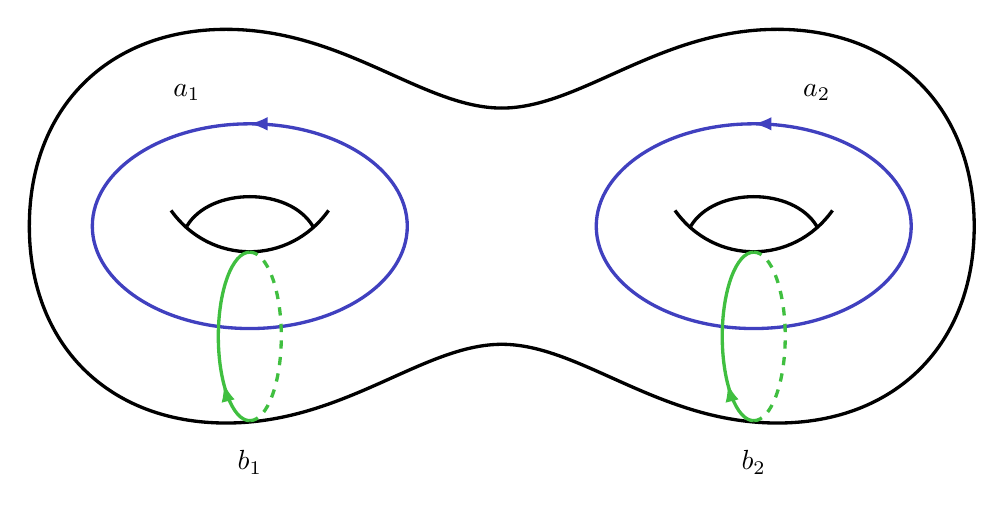
\begin{tikzpicture}
    \colorlet{darkgreen}{green!50!gray}
    \colorlet{darkblue}{blue!50!gray}

    \begin{scope}[very thick]
    % Quadrant II of Torus
    % (other draw statements are flips / rotations)
    \draw (-6,0) ..
          controls (-6,1.5) and (-5,2.5) ..
          (-3.5,2.5) ..
          controls (-2,2.5) and (-1,1.5) ..
          (0,1.5);
    \draw[xscale=-1] (-6,0) ..
          controls (-6,1.5) and (-5,2.5) ..
          (-3.5,2.5) ..
          controls (-2,2.5) and (-1,1.5) ..
          (0,1.5);
    \draw[rotate=180] (-6,0) ..
          controls (-6,1.5) and (-5,2.5) ..
          (-3.5,2.5) ..
          controls (-2,2.5) and (-1,1.5) ..
          (0,1.5);
    \draw[yscale=-1] (-6,0) ..
          controls (-6,1.5) and (-5,2.5) ..
          (-3.5,2.5) ..
          controls (-2,2.5) and (-1,1.5) ..
          (0,1.5);

    % The Holes
    % (one hole at center shifted to outsides)
    \draw[xshift=-3.2cm] (-0.8,0) ..
          controls (-0.5,0.5) and (0.5,0.5) ..
          (0.8,0);
    \draw[yscale=-1,xshift=-3.2cm] (-1,-0.2) ..
          controls (-0.5,0.5) and (0.5,0.5) ..
          (1,-0.2);

    \draw[xshift=3.2cm] (-0.8,0) ..
          controls (-0.5,0.5) and (0.5,0.5) ..
          (0.8,0);
    \draw[yscale=-1,xshift=3.2cm] (-1,-0.2) ..
          controls (-0.5,0.5) and (0.5,0.5) ..
          (1,-0.2);

    % a-cycles
    \draw[xshift=-3.2cm, darkblue, decoration={markings,
              mark=at position 0.25 with {\arrow[very thick]{latex}}},
          postaction={decorate}]
         (0,0) ellipse (2cm and 1.3cm);
    \draw[xshift=3.2cm, darkblue, decoration={markings,
              mark=at position 0.25 with {\arrow[very thick]{latex}}},
          postaction={decorate}]
         (0,0) ellipse (2cm and 1.3cm);

    % b-cycles
    \draw[xshift=-3.2cm, yshift=-2.47cm,
          darkgreen, decoration={markings,
              mark=at position 0.25 with {\arrow[very thick]{latex}}},
          postaction={decorate}]
         (0,0) arc (270:90:0.4cm and 1.07cm);
    \draw[xshift=-3.2cm, yshift=-0.33cm, dashed, darkgreen]
         (0,0) arc (90:-90:0.4cm and 1.07cm);
    \draw[xshift=3.2cm, yshift=-2.47cm,
          darkgreen, decoration={markings,
              mark=at position 0.25 with {\arrow[very thick]{latex}}},
          postaction={decorate}]
         (0,0) arc (270:90:0.4cm and 1.07cm);
    \draw[xshift=3.2cm, yshift=-0.33cm, dashed, darkgreen]
         (0,0) arc (90:-90:0.4cm and 1.07cm);

    % cycle labels
    \draw (-4,1.7)  node {$a_1$};
    \draw (4,1.7)   node {$a_2$};
    \draw (-3.2,-3) node {$b_1$};
    \draw (3.2,-3)  node {$b_2$};
    \end{scope}
  \end{tikzpicture}
  \caption{A genus $g=2$ Riemann surface $X$ with the basis cycles
    $\{a_1,a_2,b_1,b_2\}$.}
  \label{RS}
\end{figure}

These cycles form a basis for all cycles defined on the Riemann surface
and is referred to as the {\it ``homology of $X$''}. That is, every
closed curve on the Riemann surface $X$ is homeomorphic to a sum of
these $a$- and $b$-cycles. Therefore, integration about a path $\gamma
\subset X$ can be reduced to integration about the $a$- and $b$-cycles.

Another theorem tell us about the space of things we can integrate on
$X$. But first, a definition. \\

\begin{definition}
  A {\bf holomorphic differential} $\omega$ of a Riemann surface $X$ is
  a differential such that in each neighborhood $U_i \subset X$ with
  local parameter $z_i$ there exists a holomorphic function $f_i : U_i
  \to \mathbb{C}$ such that $\omega = f_i(z_i)dz_i$ on
  $U_i$. (Furthermore, given two neighborhoods $U_i$ and $U_j$ the chain
  rule is preserved under coordinate transformations on $U_i \cap U_j$.)
\end{definition}

Basically, holomorphic differentials are creatures that we can integrate
on the Riemann surface $X$. The space of all holomorphic differentials
is finite dimensional over $\CC$.

\begin{theorem}
  On a genus $g$ Riemann surface, $X$, the space of holomorphic
  differentials defined on $X$ is of dimension $g$, implying that this
  space has a basis holomorphic differentials $\omega_1, \ldots,
  \omega_g$.
\end{theorem}

In the case when $X$ is hyperelliptic, all holomorphic differentials
$\omega_1, \ldots, \omega_g$ are of the form
\begin{equation} \label{eqn: holom}
  \omega_k =  \frac{\lambda^k d \lambda}{\mu}.
\end{equation}
So, for
\begin{equation*}
  \mu^2 = P(\lambda) = \sum_{j=0}^n \beta_j \lambda^j
\end{equation*}
we have [XXX]



%==============================================================================
\section{Bloch spectra}
%==============================================================================



In looking for stationary solutions we would like the eigenfunctions to
be bounded as a function of $t$, which requires that $\mu$ is purely
imaginary.  This means bounded eigenfunctions correspond to negative
$P(\lambda) = \mu^2$.  We will call the zeros of $P(\lambda)$ $E_j$.
Thus, $P(\lambda) = \mu^2 = \prod_{j=1}^n (\lambda-E_j)$.

\begin{figure}[h]
  \centering
  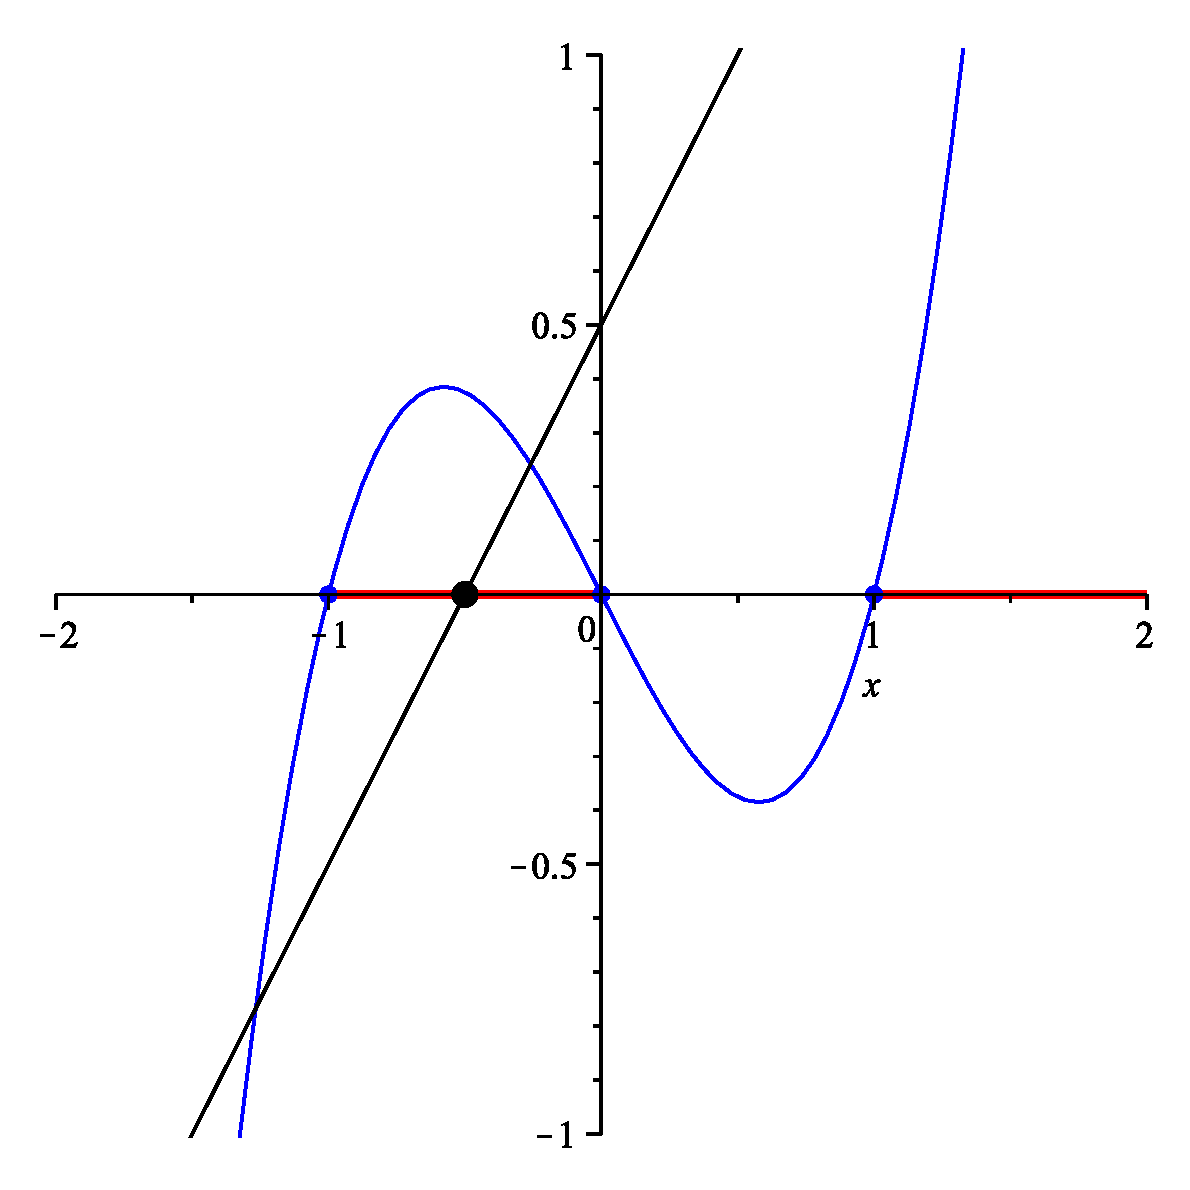
\includegraphics[scale=0.4]{./img/allowedbands.eps}\\
  \caption{Example for $n = 1$. The blue curve is $P(\lambda) = (\lambda
    - E_1)(\lambda-E_2)(\lambda-E_3)$, black curve is $b = \lambda -
    \lambda_1$. The red bands indicate forbidden bands, since
    $P(\lambda)$ is positive there. The zeros of $b(\lambda)$ always lie
    in the forbidden bands.}
  \label{fig:two}
\end{figure}

Recall that $b_n = \sum_{j=0}^n \lambda_j \beta_j$ with $\beta_n = 1$.
Since this is simply a polynomial in $\lambda$ we can write
\[
  b_n = \prod_{j=1}^n (\lambda-\lambda_j)
\]
where $\lambda_j = \lambda_j(x)$ are the zeros of $b_n$.  Then,
\[
  {b_n}_x = -\sum_{k=1}^n {\lambda_k}_x \prod_{j\neq k} (\lambda-\lambda_j).
\]
Evaluating $P(\lambda)$ at a zero of $b_n$, that is $P(\lambda_k)$ we
have
\begin{align*}
  P(\lambda_k) &=
  \mu^2
  =
  \tfrac{1}{4} {b_n}_x^2(\lambda_k) \\
  {b_n}_x(\lambda_k)
  &=
  \pm 2 \mu
\end{align*}
Then,
\begin{align*}
  \pm 2 \mu
  &=
  -{\lambda_k}_x \prod_{j\neq k} (\lambda_k - \lambda_j) \\
  {\lambda_k}_x
  &=
  \frac{\mp 2\mu}{\prod_{j\neq k} (\lambda_k - \lambda_j)} \\
  &=
  \frac{
    \mp 2 \prod_{j=1}^n (\lambda_k - E_j)^{1/2}
  }{
    \prod_{j\neq k} (\lambda_k - \lambda_j)
  }
\end{align*}

Classical Sturm Oscillation Theory tells us eigenvalues interweave since
we have a second order self-adjoint problem.  Thus, each of the
$\lambda_k$ live in their own band (bands are defined by endpoints
$E_j$) and will never collide with each other.



%==============================================================================
\section{Recovering $u(x)$}
%==============================================================================



We note that from here we can write down stationary solutions using a
related dynamical system. We have
\[
  b = \sum_{k=0}^n \beta_k \lambda^k
\]
so that
\[
  b_x = -\sum_{k=0}^n \lambda_{kx} \prod^n_{j\ne k} (\lambda - \lambda_j)
\]
and, for $\lambda = \lambda_s$
\[
  b_x = -\lambda_{sx} \prod^n_{j\ne s} (\lambda_s - \lambda_j).
\]
When $b = 0$ we have $\mu^2 = b_x^2/4$ so
\begin{align*}
  \lambda_{sx}
  &=
  \frac{
    \mp 2 \mu (\lambda_s)
  }{
    \prod^n_{j\ne s}(\lambda_s - \lambda_j)
  } \\
  &=
  \frac{
    \mp 2 \left[
      \prod_{j=1}^{2n+1} (\lambda_j - E_j)
      \right]^{1/2}
  }{
    \prod^n_{j\ne s} (\lambda_s - \lambda_j)
  }.
\end{align*}
The first step in our generating hierarchy provides
\begin{equation}\label{recover}
  2\beta_{n-1} = u + 2\gamma_{n-1},
\end{equation}
where we know
\[
  \beta_{n-1} = -\sum_{k=1}^n \lambda_k.
\]
and $\beta_n=1$. Hence knowing $\gamma_{n-1}$ in terms of the $E_j$s and
the dynamics of $\lambda_k$s we can obtain our solution $u(x)$.

Recall that given a polynomial $s(x)$ with zeros at $x_k$ we can write
$s(x) = \prod_{k=1}^n (x-x_k)$.  Also, $s(x) = x^n + \left(
-\sum_{k=1}^n x_k \right) x^{n-1} + \cdots + (-1)^n \prod_{k=1}^n x_k$
where the coefficient of the $x^{n-1}$ term is the trace of the
polynomial and the constant term is the determinant of the polynomial.

In our case, we have
\begin{align*}
  \mu^2
  &=
  \prod_{j=1}^{2n+1} (\lambda-E_j) \\
  &=
  \lambda^{2n+1} + \lambda^{2n} 2\gamma_{n-1} + \lambda^{2n-1}
  \left( 2\gamma_{n-2} + \gamma_{n-1}^2 \right) + \ldots
\end{align*}
Thus, the coefficient of $\lambda^{2n}$ must equal
$-\sum_{j=1}^{2n+1}E_j$.  So,
\[
  \gamma_{n-1} = -\frac{1}{2} \sum_{j=1}^{2n+1} E_j.
\]
Using equation \eqref{recover} we have
\begin{align*}
  u(x)
  &=
  2\beta_{n-1} - 2\gamma_{n-1} \\
  &=
  -2\sum_{k=1}^n \lambda_k - 2\gamma_{n-1} \\
  &=
  -2\sum_{k=1}^n \lambda_k + \sum_{j=1}^{2n+1} E_j.
\end{align*}

\textbf{[XXX] Why is this method not preferred? (B)}



%==============================================================================
\section{Bogoyavlenskii-Novikov}
%==============================================================================
\cite{BN, Decon}



The infinite hierarchy for KdV can be obtained using \eqref{heirarchy1},
\eqref{heirarchy2} and \eqref{nKdV}.  Also, we could find the hierarchy
by using the recursion operator $L = -\tfrac{1}{4} \partial_x^2 +
\tfrac{1}{2} \int u_x \ud x$ where
\[
  u_{t_n} = \partial_x(L^n u).
\]
Also, we could present the hierarchy in a form using variational
derivatives:
\[
  u_{t_n} = \partial_x \frac{\delta I_n}{\delta u}
\]
with $I_n$ being the $n$-th conserved quantity of KdV and defined as
$I_n = \int Q_n(u,u_x,\ldots {u_n}_x) \ud x$.

We state theorems (without proof) related to this method.

\begin{theorem}{\cite{Lax}}
  The set of stationary solutions of the $n$-th KdV equation is
  invariant under the other KdV flows.
\end{theorem}
We will call
\[
  u_t = \partial_x \frac{\delta}{\delta u}
  \left(
  I_n + c_1 I_{n-1} + \ldots + c_n I_0
  \right)
\]
the $n$-th KdV equation. Novikov showed \cite{Nov} that every genus $g$
solution of KdV 1 is a stationary solution of the $g$-th KdV equation.
We will consider the $n$-th stationary KdV equation given by
\[
  \frac{\delta}{\delta u}
  \left(
  I_n + c_1 I_{n-1} + \cdots + c_n I_0 + c_{n+1}I_{-1}
  \right)=0
\]
where $I_{-1}=\int u \ud x$.

We define
\[
  S = I_n + c_1 I_{n-1} + \cdots + c_n I_0 + c_{n+1}I_{-1} =\int L \ud x
\]
with Langrangian
\[
  L = Q_n + c_1Q_{n-1} + \cdots + c_n Q_0 + c_{n+1} Q_{-1}
\]
and introduce new variables,
\begin{align*}
  q_i
  &= u^{(i-1)} \\
  p_1
  &=
  \pp{L}{u'} - \frac{\ud}{\ud x} \pp{L}{u''} +
  \cdots + (-1)^{n-1} \frac{\ud^{n-1}}{\ud x^{n-1}}
  \pp{L}{u^{(n)}}
  =
  \frac{\delta S}{\delta u'} \\
  p_2
  &=
  \pp{L}{u''} - \frac{\ud}{\ud x} \pp{L}{u'''} +
  \cdots + (-1)^{n-2} \frac{\ud^{n-2}}{\ud x^{n-2}}
  \pp{L}{u^{(n)}}
  =
  \frac{\delta S}{\delta u''} \\
  & \vdots \\
  p_n
  &=
  \pp{L}{u^{(n)}}
  =
  \frac{\delta S}{\delta u^{(n)}}.
\end{align*}

\begin{theorem}[Ostrogradskii \cite{Ost}]
  The Euler-Langrange equation for a Lagrangian $L = L(u, u', \ldots,
  u^{(n)})$, which is nonsingular, is equivalent to the Hamiltonian
  system
  \[
    q_i' = - \pp{H}{p_i},  \quad p_i' = \pp{H}{q_i}, [XXX]
  \]
  with $H(q,p) = p_1u' + p_2u'' + \cdots + p_n u^{(n)}-L$.
\end{theorem}

\begin{theorem}
  The Hamiltonian $H$ from Ostrogradskii's theorem is related to the
  action $S$ through $H'=-u' \frac{\delta S}{\delta u}$.
\end{theorem}

\begin{theorem}[Bogoyavlenskii-Novikov \cite{BN} ]
  On the solution space of the $n$-th stationary KdV equation, the
  $i$-th KdV flow, $u_{t_i} = \partial_x \left( \frac{\delta I_i}{\delta
    u} \right)$, (without adding in the lower flows) can be written as a
  Hamiltonian system with Hamiltonian $H_i = -T_i$ and the same
  canonical variables as determined by Ostrogradskii's theorem for the
  $n$-th order spatial system.
\end{theorem}



%==============================================================================
\section{The Riemann-theta function representation}
%==============================================================================



Alternatively we can cast the problem in terms of Riemann theta
functions...  [XXX]

Let's return to the eigenvetors of the operator $T_n$. As seen in
Section \ref{sec: bloch} the eigenvectors $\phi$ are of the form
\begin{equation*}
  \phi(x)
  =
  \frac{1}{\mu-a_n(x_0)} \sqrt{\frac{b_n(x_0)}{b_n(x)}}
  \exp \left( \mu \int_{x_0}^x \frac{dx}{b_n} \right)
  \begin{pmatrix}
    b_n \\ \mu-a_n
  \end{pmatrix}
\end{equation*}
after renormalization about some base



%%%%%%%%%%%%%%%%%%%%%%%%%%%%%%%%%%%%%%%%%%%%%%%%%%%%%%%%%%%%%%%%%%%%%%%%%%%%%%%
\newpage
\appendix
%%%%%%%%%%%%%%%%%%%%%%%%%%%%%%%%%%%%%%%%%%%%%%%%%%%%%%%%%%%%%%%%%%%%%%%%%%%%%%%



%==============================================================================
\section{Code}\label{code}
%==============================================================================



A Rosetta stone of symbolic mathematics...

\textbf{Mathematica:}
\begin{align*}
&n=5;\\
&b\text{[x\_}]=\text{Sum}\left[\beta _j[x]\lambda ^j,\{j,0,n\}\right];\\
&\beta _n[\text{x\_}]=1;\\
&\text{Do}\left[\beta _{i-1}[\text{x$\_$}]=\gamma _{i-1}+\text{Integrate}\left[\frac{1}{2}\text{D}\left[u\left[x,t_n\right],x\right]\beta _i[x]+\frac{1}{4}\beta _i'''[x]+u\left[x,t_n\right]\beta _i'[x],x\right],\{i,n,0,-1\}\right]\\
&\text{KdV}[n]=\text{Expand}\left[\text{D}\left[u\left[x,t_n\right],x\right]\beta _0[x]+\frac{1}{2}\beta _0'''[x]+2u\left[x,t_n\right]\beta _0'[x]- \text{D}\left[u\left[x,t_n\right],t_n\right]\right]\\
&T_n[\text{x$\_$}]=\left\{\left\{\frac{-1}{2}b'[x],b[x]\right\},\left\{\left(\lambda -u\left[x,t_n\right]\right)b[x]-\frac{1}{2}b''[x],\frac{1}{2}b'[x]\right\}\right\};\\
&P[\lambda \_,\text{x$\_$}]=-\text{Collect}\left[\text{Det}\left[T_n[x]\right],\lambda \right]\\
&\text{Coefficient}\left[P[\lambda ,x],\lambda ^{2n+1}\right]\\
&\text{Coefficient}\left[P[\lambda ,x],\lambda ^{2n}\right]\\
&\text{Coefficient}\left[P[\lambda ,x],\lambda ^{2n-1}\right]\\
&\text{Coefficient}\left[P[\lambda ,x],\lambda ^{2n-2}\right]\\
&\text{Coefficient}\left[P[\lambda ,x],\lambda ^{2n-3}\right]\\
&\text{Coefficient}\left[P[\lambda ,x],\lambda ^{2n-4}\right]\\
&\text{Coefficient}\left[P[\lambda ,x],\lambda ^{2n-5}\right]\\
&\text{Coefficient}\left[P[\lambda ,x],\lambda ^{2n-6}\right]\\
\end{align*}

\textbf{Maple:} The following lines compute $P(\lambda)$ for a specified
$n$. Here $n = 1$. The first constant $\gamma_1$ is arbitrary and here
is set to $\gamma_1 = 4$ to give the desired coefficients for the first
KdV flow.
\begin{verbatim}
> restart; with(LinearAlgebra);
> T := Matrix([[A, B], [C, -A]]);
> n := 1;
> beta[n] := 4;
> for k from 1 to n do
    j := n-k;
    beta[j] := (1/2)*(int((1/2)*(diff(beta[j+1], `$`(x, 3)))...
    +2*u(x)*(diff(beta[j+1], x))+(diff(u(x), x))*beta[j+1], x))+gamma[j]
  end do;
> nflow := expand((1/2)*(diff(beta[0], `$`(x, 3)))+2*u(x)*(diff(beta[0], x))...
    +(diff(u(x), x))*beta[0]);
> B := sum(lambda^i*beta[i], i = 0 .. n);
> A := -(1/2)*(diff(B, x));
> C := diff(A, x)+B*(lambda-u(x));
> P := A^2+B*C;
> collect(simplify(P), [lambda, gamma[1]]);
\end{verbatim}

\textbf{Python:}



%==============================================================================
\section{Independence of $T$ for the Stationary Flow}\label{det/trace}
%==============================================================================



\textbf{THIS SECTION NEEDS HELP...}


Given
\[
  T_x +T X = XT + X_t
\]
with $X=X(x,t),T=T(x,t)$ matrices we note that for the stationary flow,
$X_t=0$.  We would like to show that $T_x=0$. Our equation is equivalent to 
\[
  T_x = [X,T]
\]
where $[\cdot,\cdot]$ is the usual matrix commutator. Taking the trace
of both sides, we have
\[
  \pp{}{x} \left( \tr(T) \right) = \tr[X,T] = 0
\]
since the trace is cyclic (that is $\tr(AB) = \tr(BA)$).  Thus, $T$ is
independent of $X$.

Now, observe that
\begin{align*}
  TT_x &= T(XT-TX) \\
       &= TXT-T^2X \\
       &= [TX,T],
\end{align*}
\begin{align*}
  T^n[X,T] &= T^n(XT-TX) \\
           &= T^nXT - T^{n+1}X \\
           &= [T^nX, T],
\end{align*}
and similarly,
\[
  T_x T = [XT,T].
\]
Now,
\begin{align*}
  \pp{}{x}T^2 &= \pp{}{x} \left(T \cdot T \right) \\
              &= TT_x + T_xT \\
              &= [XT+TX, T]
\end{align*}
so $\pp{}{x}(\tr (T^2))=0$. Similarly,
\begin{align*}
  \pp{}{x}T^n &= \sum_{k=1}^n T^{n-k} T_x T^{k-1} \\
              &= \left[ \sum_{k=1}^n T^{n-k} X T^{k-1}, T \right]
\end{align*}
and $\pp{}{x}(\tr (T^n))=0$.



%%%%%%%%%%%%%%%%%%%%%%%%%%%%%%%%%%%%%%%%%%%%%%%%%%%%%%%%%%%%%%%%%%%%%%%%%%%%%%%
\newpage
\bibliographystyle{plain}
\begin{thebibliography}{99}
%%%%%%%%%%%%%%%%%%%%%%%%%%%%%%%%%%%%%%%%%%%%%%%%%%%%%%%%%%%%%%%%%%%%%%%%%%%%%%%


\bibitem{BN} O.I. Bogoyavlenskii and S.P. Novikov. The relationship
  between Hamiltonian formalisms of stationary and nonstationary
  problems. \emph{Funct. Anal. Appl.}, 10:8-11, 1976.

\bibitem{Decon} B. Deconinck (Ph.D. thesis). The Initial-Value Problem
  for Multiphase Solutions of the Kadomtsev-Petviashvili
  Equation. University of Colorado at Boulder 1998.

\bibitem{Ost} B.A. Dubrovin, A.T. Fomenko, and S.P. Novikov. Nonlinear
  equations of Korteweg-de Vries type, finite-band linear operators and
  Abelian varieties. \emph{Russian Math. Surveys}, 31(1):59-146, 1976.

\bibitem{Lax} P.D. Lax. Periodic Solutions of the KdV
  equation. \emph{Comm. pure Appl. Math.}, 28:141-188, 1975.

\bibitem{Nov} S.P. Novikov. A periodic problem for the Korteweg-de Vries
  equation. I. \emph{Funct. Anal. Appl.,} 9:236-246, 1974.

\end{thebibliography}
\end{document}
